\section{Understanding Rollup.c}
One of the predominant optimizations in GUFI is the rollup feature which functions like so: \\
\begin{itemize}
  \item Contents of the child's summary table are copied up with name column to include the parent directory
  \item Pentries view/table is dropped and a pentries table is created with the data inside the pentries view/table
  \item Copy child's pentries view into parent (regardless if view or table)
  \item All children must be able to rollup
\end{itemize}


\begin{figure} [h]
\centering
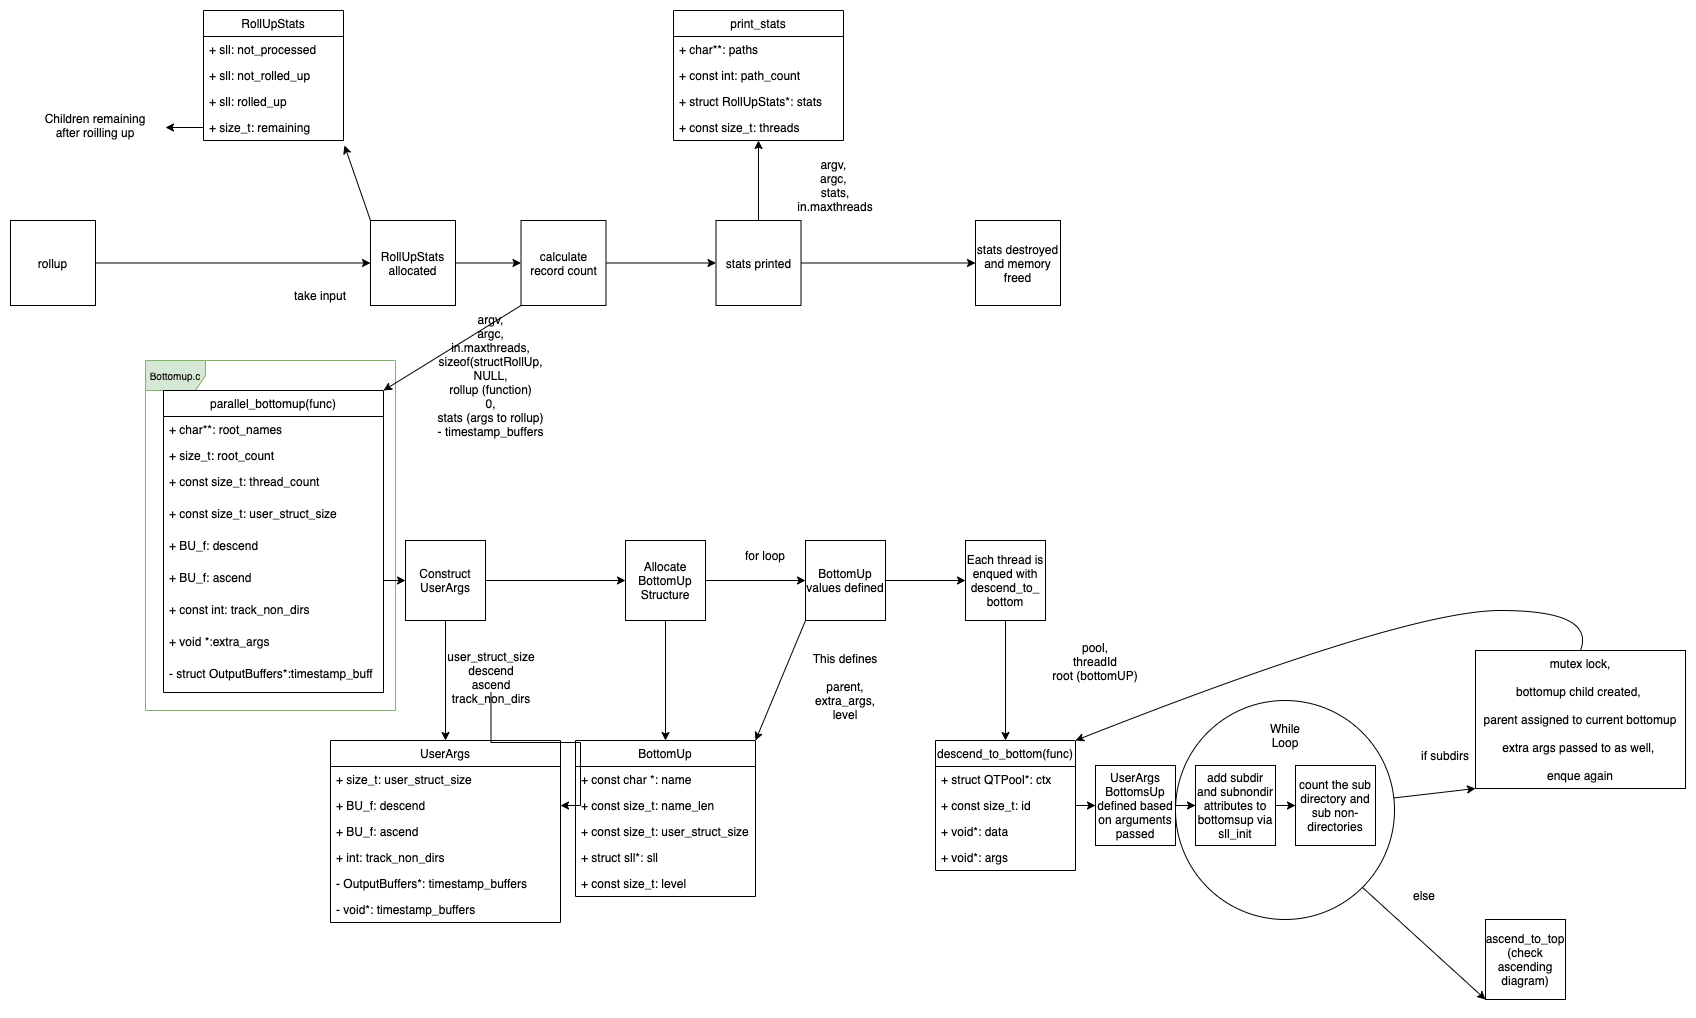
\includegraphics[width=1.2\textwidth]{images/rollup.png}
\caption{\label{fig:rollup}Rollup.c Workflow}
\end{figure}

\clearpage

\subsection{\texttt {ascend\_to\_top}}
ascend\_to\_top is a versatile function that will perform a function as it ascends the tree.

\begin{figure} [h]
\centering
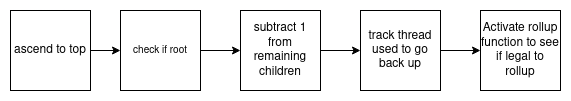
\includegraphics[width=0.8\textwidth]{images/ascending.png}
\caption{\label{fig:ascending_diagram} Ascending Diagram}
\end{figure}

In this case, we will be passing in the rollup function inside of \texttt{rollup.c}.

\begin{figure} [h]
\centering
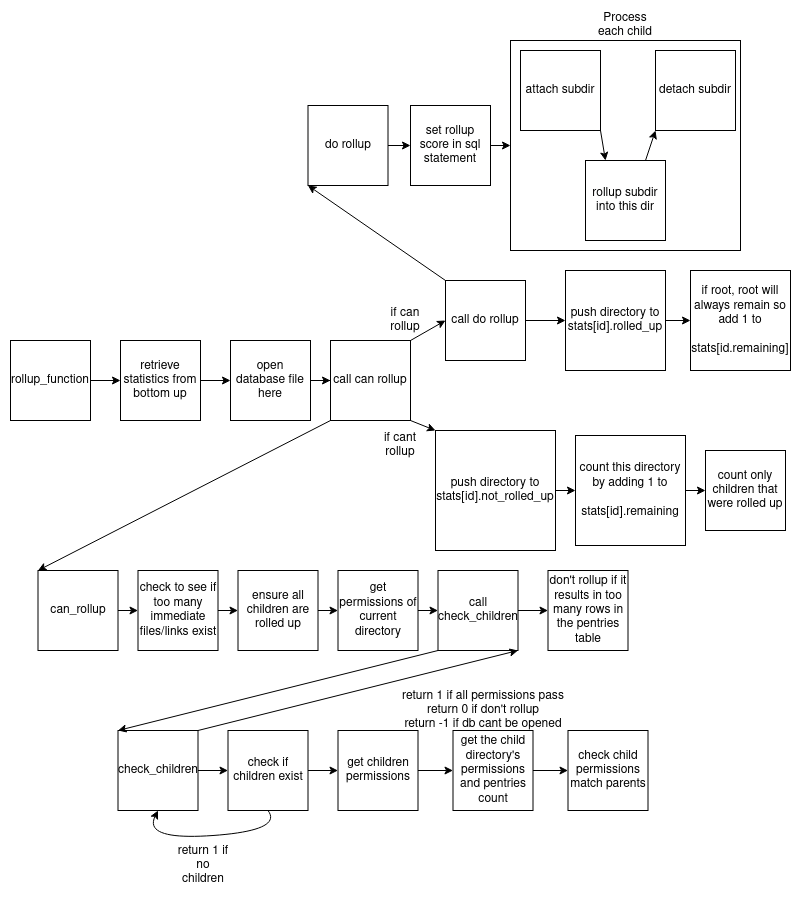
\includegraphics[height=0.45\textheight]{images/rollup_function.png}
\caption{\label{fig:rollup_function} Rollup Function Diagram}
\end{figure}

\clearpage